% Results section (Sachin). Paste into the IEEE Overleaf project after Methodology / Feature Engineering.
% Needs \usepackage{graphicx}. Figures are in reports/figures/ (upload them to a figures/ folder in Overleaf).
% New BibTeX key used here: lundberg2017 (Lundberg & Lee, "A Unified Approach to Interpreting Model
% Predictions", NeurIPS 2017). Other keys (huot2022, chen2016, ke2017) are already in the methodology draft.
% Every number below comes from notebooks/02_evaluation.ipynb and reports/results.csv.

\section{Results}

All models are scored on the same 6.73\,M labelled test pixels (1\,689 patches), of which 1.25\% burn on
day $t+1$. Pixels labelled $-1$ are excluded throughout. Precision, recall and F1 use the threshold that
maximises F1 on the eval split; PR AUC, ROC AUC and recall at a fixed false positive rate (FPR) need no threshold.

\subsection{Overall performance}

Table~\ref{tab:results} and Fig.~\ref{fig:pr} summarise the six models. The tuned XGBoost on all 35 features
is the best model on every threshold-free metric (PR AUC 0.256, ROC AUC 0.903), with LightGBM practically
tied (0.252). Both clearly beat every model trained on the 12 raw channels (PR AUC 0.145--0.157) and the
persistence baseline (0.106). Since the two boosting libraries reach almost the same score while the
raw-channel XGBoost scores 0.145, the gain comes from the engineered features rather than from the learner.

\begin{table*}[t]
\centering
\caption{Test results. Precision, recall and F1 at the threshold chosen on the eval split.
Bottom: PR AUC reported by Huot et al.~\cite{huot2022} on the same test split, for reference only
(their logistic regression and random forest also receive the 8 neighbouring pixels of every channel).}
\label{tab:results}
\begin{tabular}{lccccccc}
\hline
Model & PR AUC & ROC AUC & Precision & Recall & F1 & Recall @ 1\% FPR & Recall @ 5\% FPR \\
\hline
Persistence & 0.106 & 0.633 & 0.357 & 0.273 & 0.309 & 0.273 & 0.273 \\
Logistic regression (raw) & 0.146 & 0.798 & \textbf{0.378} & 0.266 & 0.312 & 0.281 & 0.319 \\
Random forest (raw) & 0.157 & 0.816 & 0.371 & 0.270 & 0.312 & 0.279 & 0.362 \\
XGBoost (raw) & 0.145 & 0.795 & 0.337 & 0.257 & 0.292 & 0.267 & 0.375 \\
XGBoost (tuned, all features) & \textbf{0.256} & \textbf{0.903} & 0.257 & 0.504 & \textbf{0.341} & \textbf{0.390} & \textbf{0.675} \\
LightGBM (tuned, all features) & 0.252 & 0.896 & 0.253 & \textbf{0.514} & 0.339 & 0.389 & 0.670 \\
\hline
\multicolumn{8}{l}{\emph{Huot et al.~\cite{huot2022}:} persistence 0.115, logistic regression 0.198,
random forest 0.225, convolutional autoencoder 0.284 (PR AUC).} \\
\hline
\end{tabular}
\end{table*}

\begin{figure}[t]
\centering
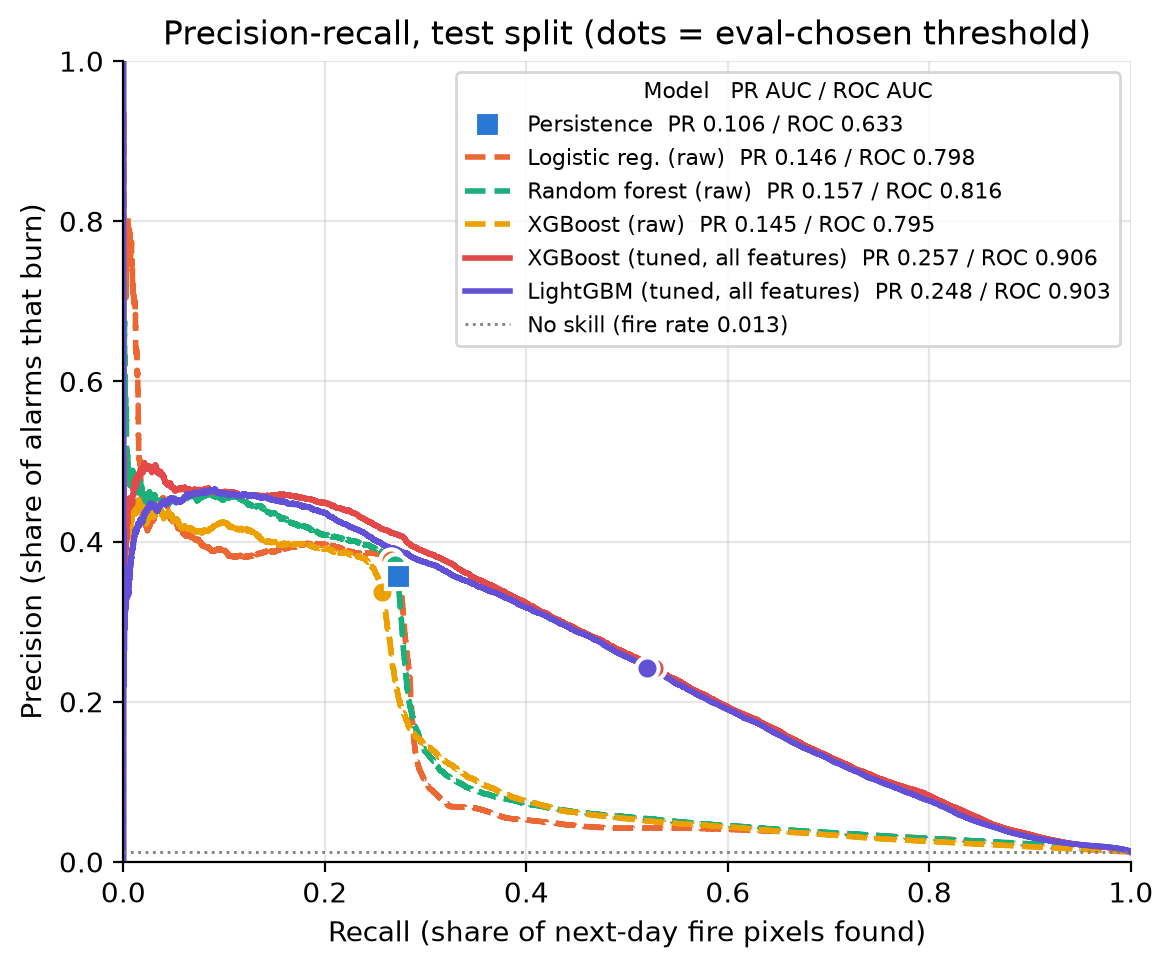
\includegraphics[width=\columnwidth]{figures/eval_pr_curves.png}
\caption{Precision--recall curves on the test split. Dots mark each model's eval-chosen threshold;
persistence outputs only 0/1 and is a single point (square).}
\label{fig:pr}
\end{figure}

\textbf{PR vs.\ ROC.} With 79 non-fire pixels per fire pixel, ROC AUC is high for every learned model
(0.80--0.90) while PR AUC stays below 0.26: a false alarm barely moves the false positive rate but directly lowers
precision. A random ranking scores 0.5 ROC AUC but only 0.0125 PR AUC, which is why PR AUC is our main metric.

\textbf{What the baselines learn.} The raw-channel models keep 0.35--0.45 precision up to a recall of 0.27,
which is the recall of persistence, and then collapse to about 0.05 (Fig.~\ref{fig:pr}). They rank pixels that are
already burning first and have almost no signal for new fire, so at their operating point they are no better than
persistence (F1 0.29--0.31 vs.\ 0.31). The tuned models keep 0.25--0.45 precision up to a recall of 0.50 and
are the only models that find a large share of newly burning pixels.

\textbf{Operating point.} At the eval-chosen threshold the tuned XGBoost finds half of all next-day fire
(recall 0.504) at precision 0.257, about twice the recall of any baseline; F1 is 0.341, close to the
test-optimal 0.359, so the threshold transfers well from eval to test. At a fixed FPR of 1\% and 5\% it finds
39\% and 67\% of fire pixels, while persistence is stuck at 27\%. At persistence's own FPR (0.62\%) XGBoost
finds 31\% of fire pixels against 27\%.

\textbf{Comparison with Huot et al.} Our persistence baseline (0.106) is close to theirs (0.115), which supports
the pipeline. The tuned XGBoost (0.256) exceeds their random forest with neighbour features (0.225) but stays below
their convolutional autoencoder (0.284). These numbers come from different pipelines and are a reference, not a
controlled comparison; they suggest that engineered neighbourhood features close most, but not all, of the gap to a
spatial model.

\subsection{Probability maps}

Fig.~\ref{fig:maps} shows ten test patches drawn at random (seed 0) among those with next-day fire.
The predicted probability is a smooth halo around the day-$t$ fire that fades over 2--5\,km, and its shape follows
the day-$t$ mask rather than the wind direction. After thresholding, the prediction is close to the day-$t$ fire
grown by about 2\,km: fire that persists or creeps outward is caught, small fires that die down leave a ring of
false positives, and fire appearing away from the day-$t$ fire is missed. The probabilities are not calibrated
(training on a 1:5 subsample with \texttt{scale\_pos\_weight}\,$\approx$\,5 raises all of them, hence the high
threshold of 0.92); only their ranking is used.

\begin{figure*}[t]
\centering
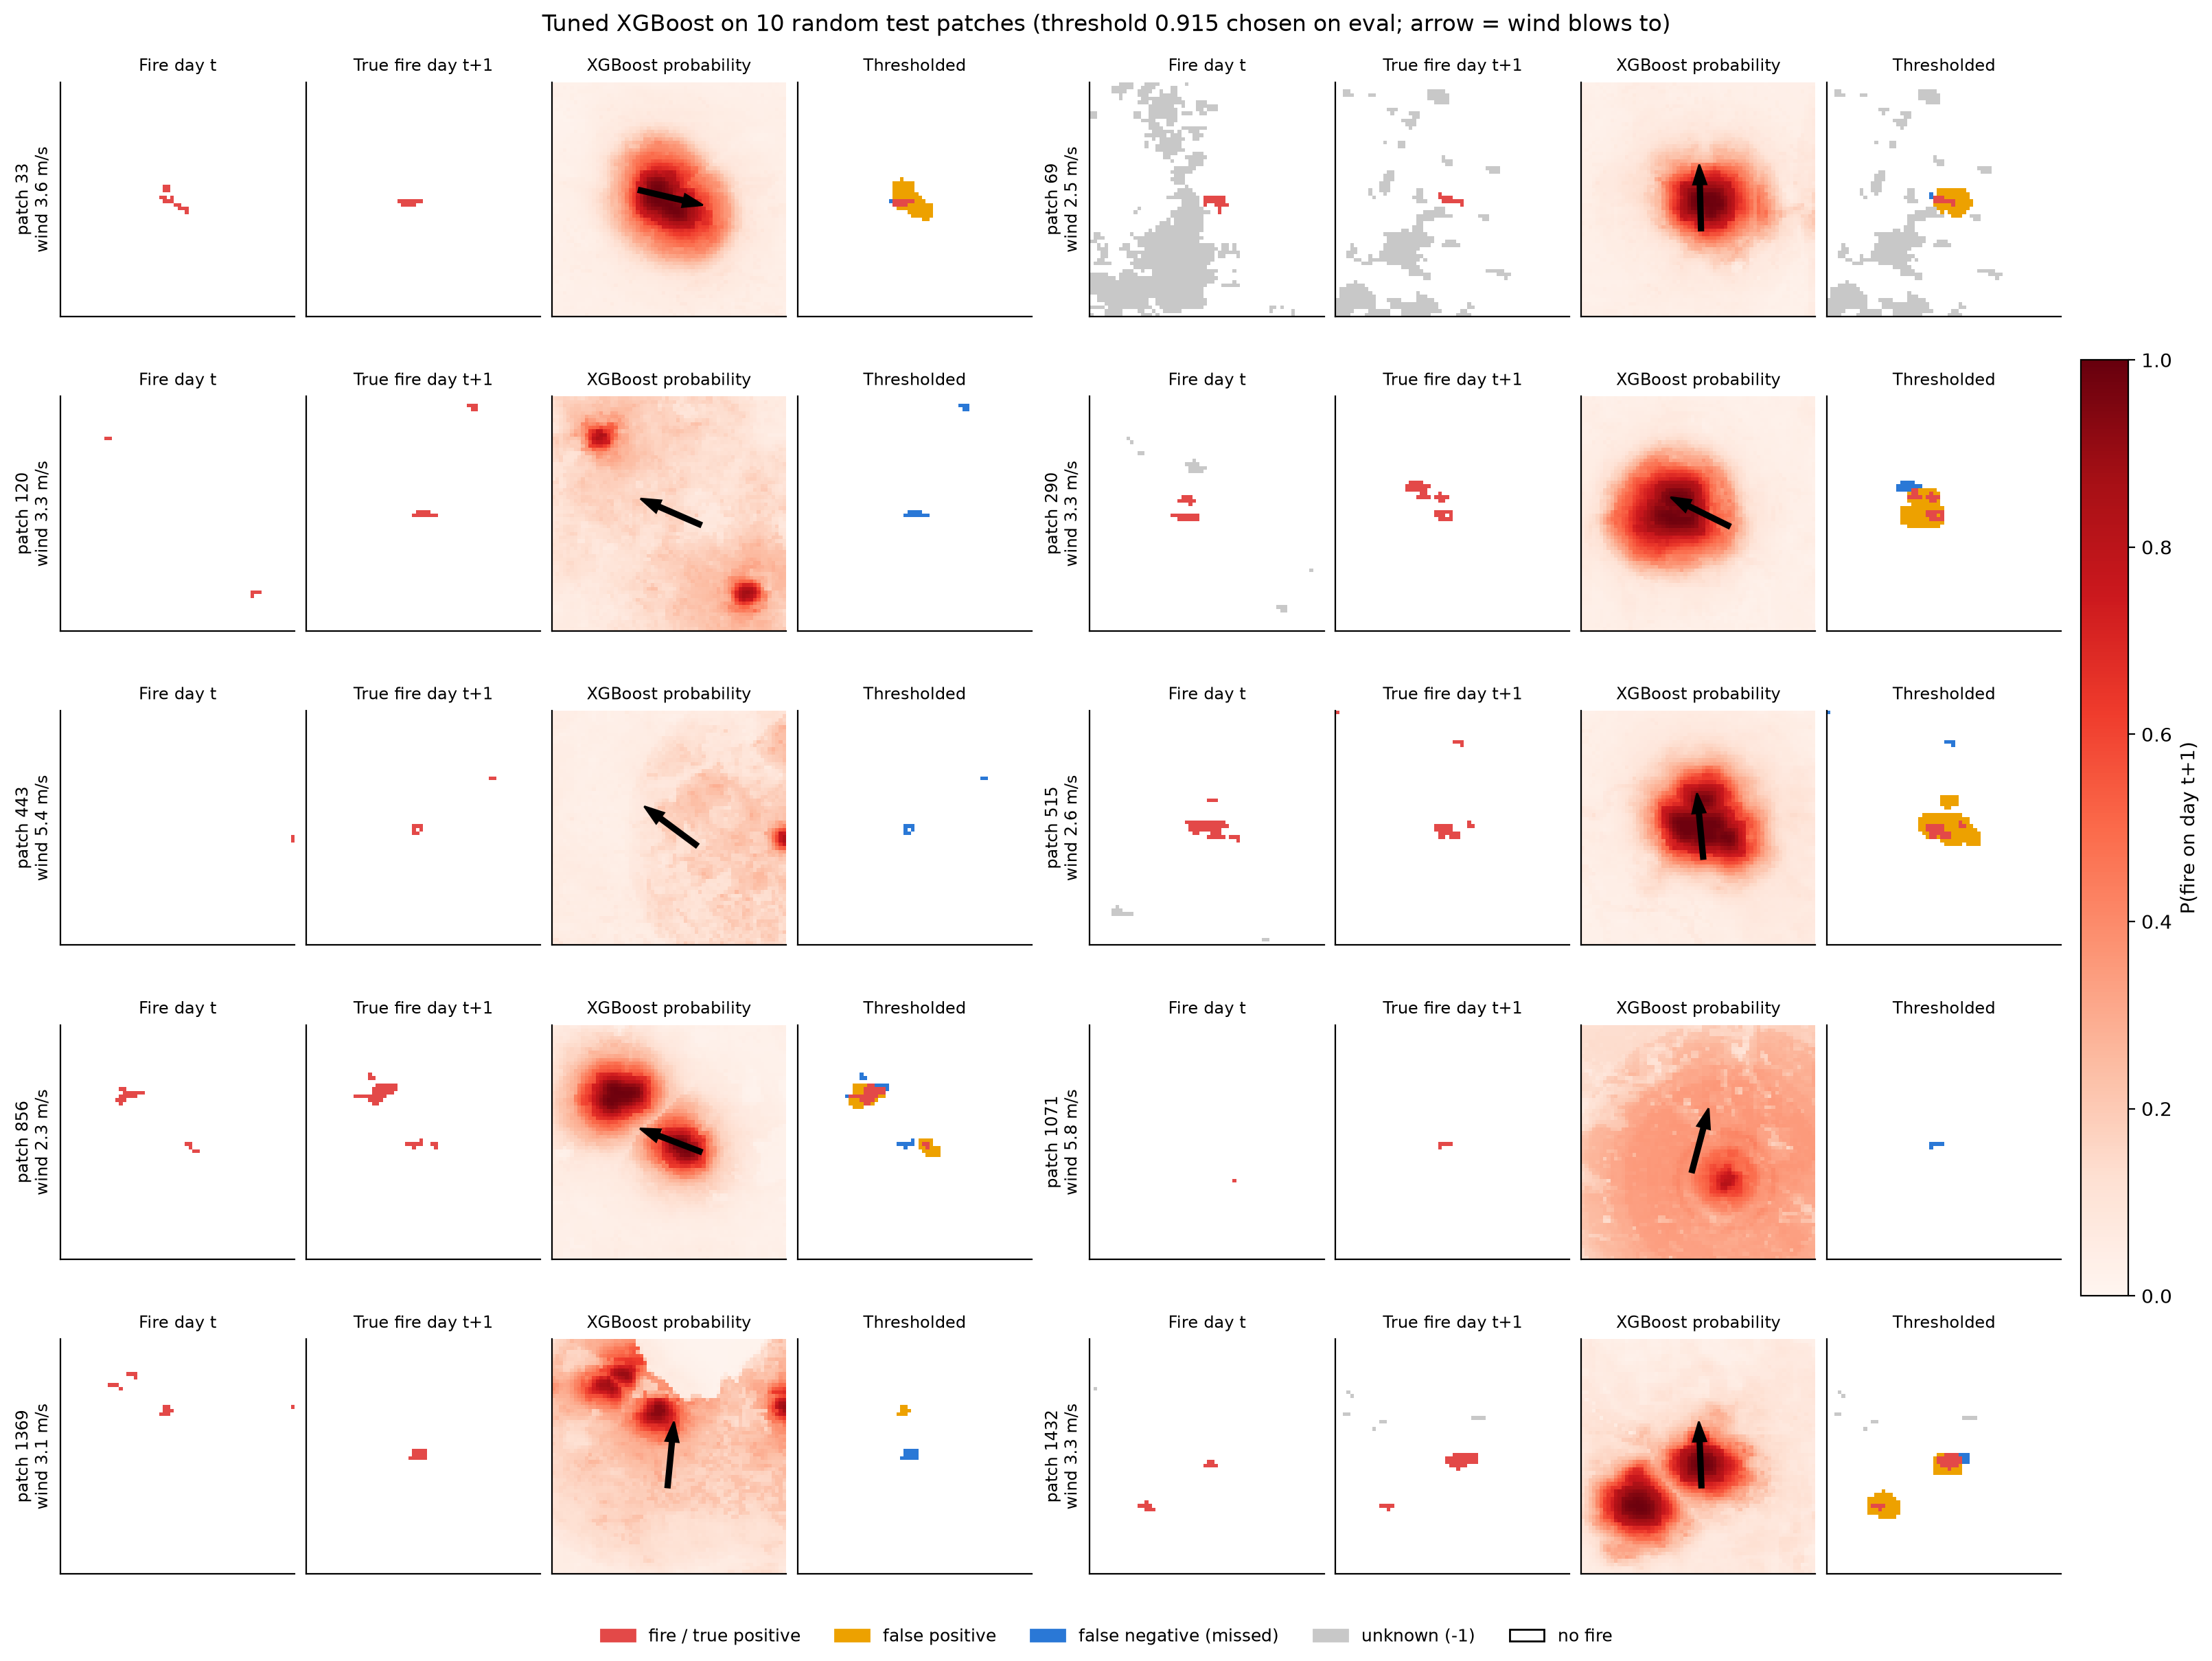
\includegraphics[width=\textwidth]{figures/eval_prob_maps.png}
\caption{Tuned XGBoost on ten random test patches. Per patch: day-$t$ fire, true day-$t{+}1$ fire, predicted
probability (arrow: direction the wind blows to), and thresholded prediction coloured by outcome.
Grey: label $-1$.}
\label{fig:maps}
\end{figure*}

\subsection{Feature importance and SHAP}

To explain the tuned XGBoost we refit it with the stored hyperparameters; it reproduces the evaluated test
predictions exactly. Fire-neighbourhood features dominate: \texttt{dist\_to\_fire} (34\% of total gain),
\texttt{prev\_fire\_n9} (22\%) and \texttt{prev\_fire\_n5} (14\%) together hold 70\% of the gain, and the eight
fire features in the top 15 hold 84\%. SHAP values~\cite{lundberg2017}, computed exactly with TreeExplainer on
20\,000 test pixels (10\,000 fire, 10\,000 non-fire), agree (Fig.~\ref{fig:shap}): the fire-neighbourhood group
contributes 2.30 log-odds on average against 0.43 for all weather features, 0.24 for vegetation, 0.21 for terrain
and 0.14 for human features. \texttt{dist\_to\_fire} alone moves a prediction from about $+2.5$ log-odds at the fire
to $-2.5$ beyond 40\,km.

\begin{figure}[t]
\centering
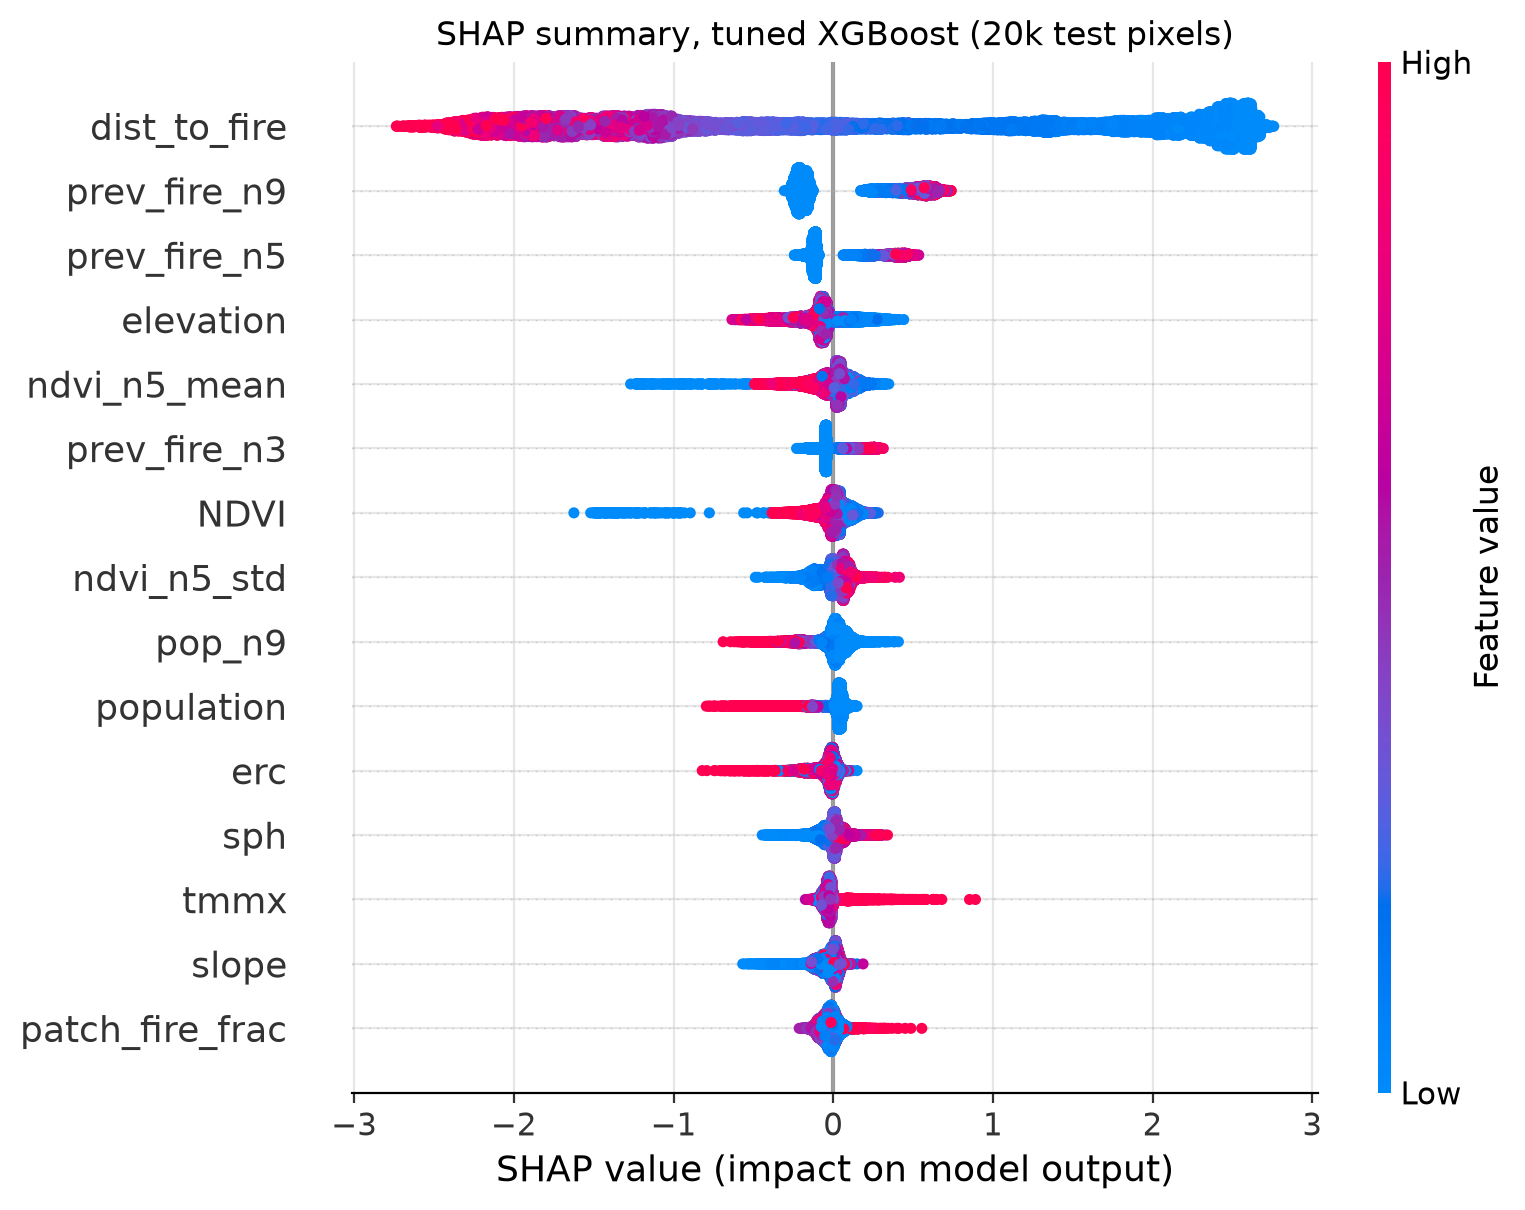
\includegraphics[width=\columnwidth]{figures/eval_shap_summary.png}
\caption{SHAP summary for the tuned XGBoost (top 15 features, 20k test pixels). Positive values push toward fire.}
\label{fig:shap}
\end{figure}

\subsection{Physical plausibility}

Most effects match fire physics (Spearman $\rho$ between a feature and its SHAP value in brackets).
Risk rises closer to fire ($\rho=-0.97$ for \texttt{dist\_to\_fire}), with more fire nearby, with fire upwind
(\texttt{upwind\_fire\_k2/k4/k8}: $+0.69/+0.61/+0.47$), with vapour pressure deficit ($+0.75$), maximum temperature
and wind speed ($+0.79$), and falls with minimum relative humidity ($-0.63$), in sparse vegetation (low NDVI) and in
densely populated pixels. Two effects are not plausible as causes: high energy release component and high specific
humidity push toward \emph{lower} and \emph{higher} risk respectively. Both are coarse (4\,km) regional values that are
nearly constant within a patch, so the model most likely uses them as proxies for region and season;
\texttt{min\_rel\_humidity} carries the physically correct humidity effect.

\begin{figure}[t]
\centering
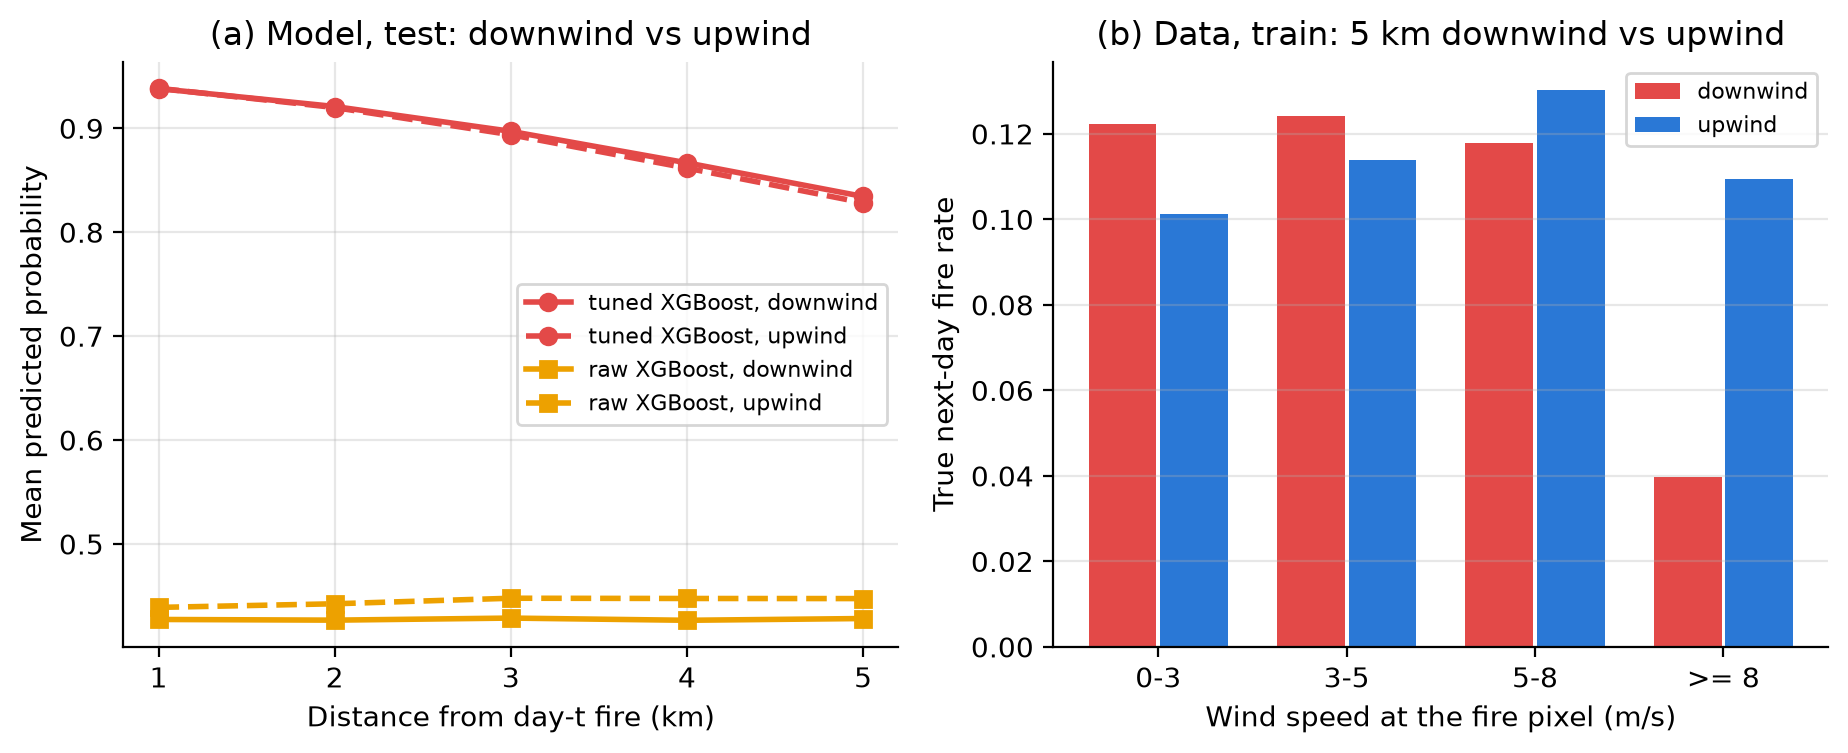
\includegraphics[width=\columnwidth]{figures/eval_downwind_check.png}
\caption{(a) Mean predicted probability 1--5\,km downwind vs.\ upwind of day-$t$ fire (test).
(b) True next-day fire rate 5\,km downwind vs.\ upwind, by wind speed (train).}
\label{fig:wind}
\end{figure}

\textbf{Does the model push risk downwind?} For every day-$t$ fire pixel we step 1--5 pixels downwind and upwind
(wind direction $\theta$ taken as the direction the wind blows from, patches north-up) and compare pixels not yet
burning. The model's mean probability differs by less than 0.006 between the two sides at every distance
(Fig.~\ref{fig:wind}a): it does \emph{not} push risk downwind, and the three upwind features have a mean $|$SHAP$|$ of only
0.005--0.012 log-odds (vs.\ 1.61 for \texttt{dist\_to\_fire}). The data explain why (Fig.~\ref{fig:wind}b): under winds below 5\,m/s next-day fire is
9--21\% more frequent 5\,km downwind, as expected, but under winds of 8\,m/s or more it is 2.7 times more frequent on
the \emph{upwind} side (0.109 vs.\ 0.040), and the test split shows the same reversal. Strong winds are where direction
should matter most, so either the direction convention assumed for this export is flipped, or a confounder
(e.g.\ strong offshore winds driving fire toward unburnable land) dominates. In both cases the hand-coded upwind
features carry mixed signal; we flag the convention for verification in Phase~2, where a CNN can learn the relation
between the wind field and the fire front directly.

\subsection{Error analysis}

At the eval-chosen threshold the tuned XGBoost produces 42.5\,k true positives, 123.0\,k false positives and
41.8\,k false negatives. We inspected the five test patches with the most false-positive and the most false-negative
pixels (Fig.~\ref{fig:errors}), keeping one patch per location because the dataset contains several overlapping
crops of the same large fire.

\textbf{False positives} come from large, fragmented fires that are dying down. All five worst patches contain
255--468 burning pixels on day $t$, and in four of them the fire shrinks by 40--60\% the next day; the model draws its
2\,km halo around every burning pixel regardless. Across the test split only 35\% of day-$t$ fire pixels still burn
on day $t+1$, 93\% of false positives lie within 2\,km of day-$t$ fire, and 54\% fall in shrinking patches although only
38\% of patches shrink. The inputs carry no information on burnt-out fuel, containment or next-day weather.

\textbf{False negatives} come from long-range spread and explosive growth: new fire 10--40\,km from the day-$t$ fire
(in one case partly hidden by cloud on day $t$) and a fire growing from 8 to 260 pixels in one day. Recall falls
sharply with distance from the day-$t$ fire (Fig.~\ref{fig:dist}): 0.98 for pixels already burning, 0.95 at 1\,km,
0.48 at 2\,km, and below 0.02 from 3\,km on, although 43\% of next-day fire lies 3\,km or more away.
No fire pixel beyond 5\,km is found, and 61.5\% of all missed pixels lie there.

\begin{figure*}[t]
\centering
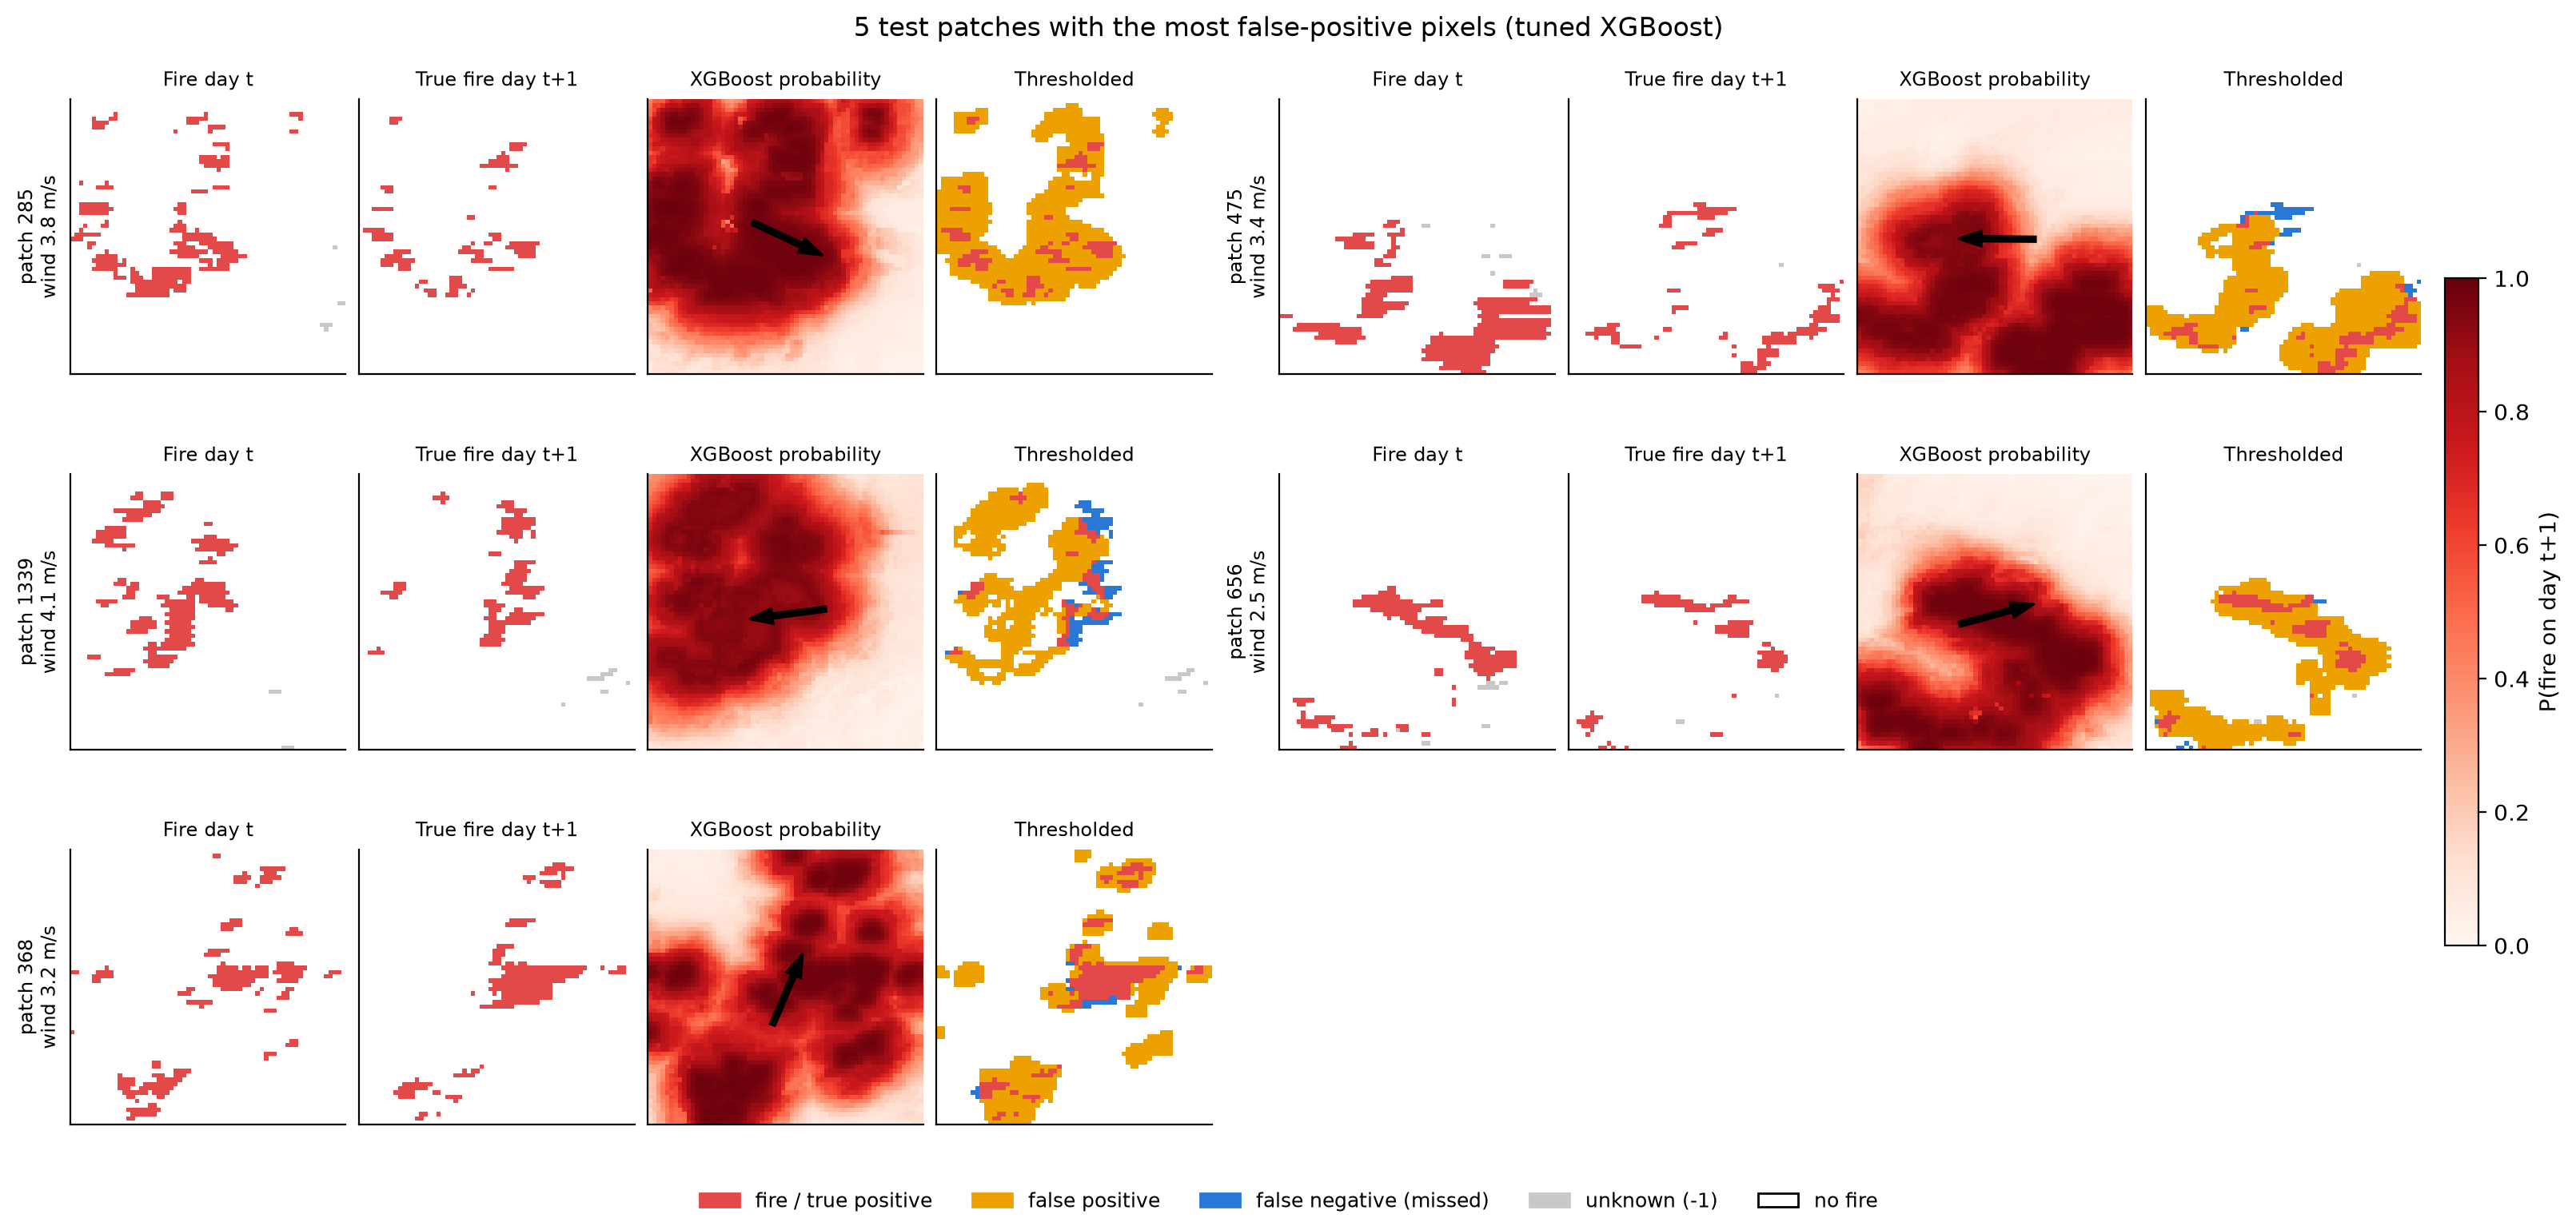
\includegraphics[width=0.49\textwidth]{figures/eval_worst_fp.png}\hfill
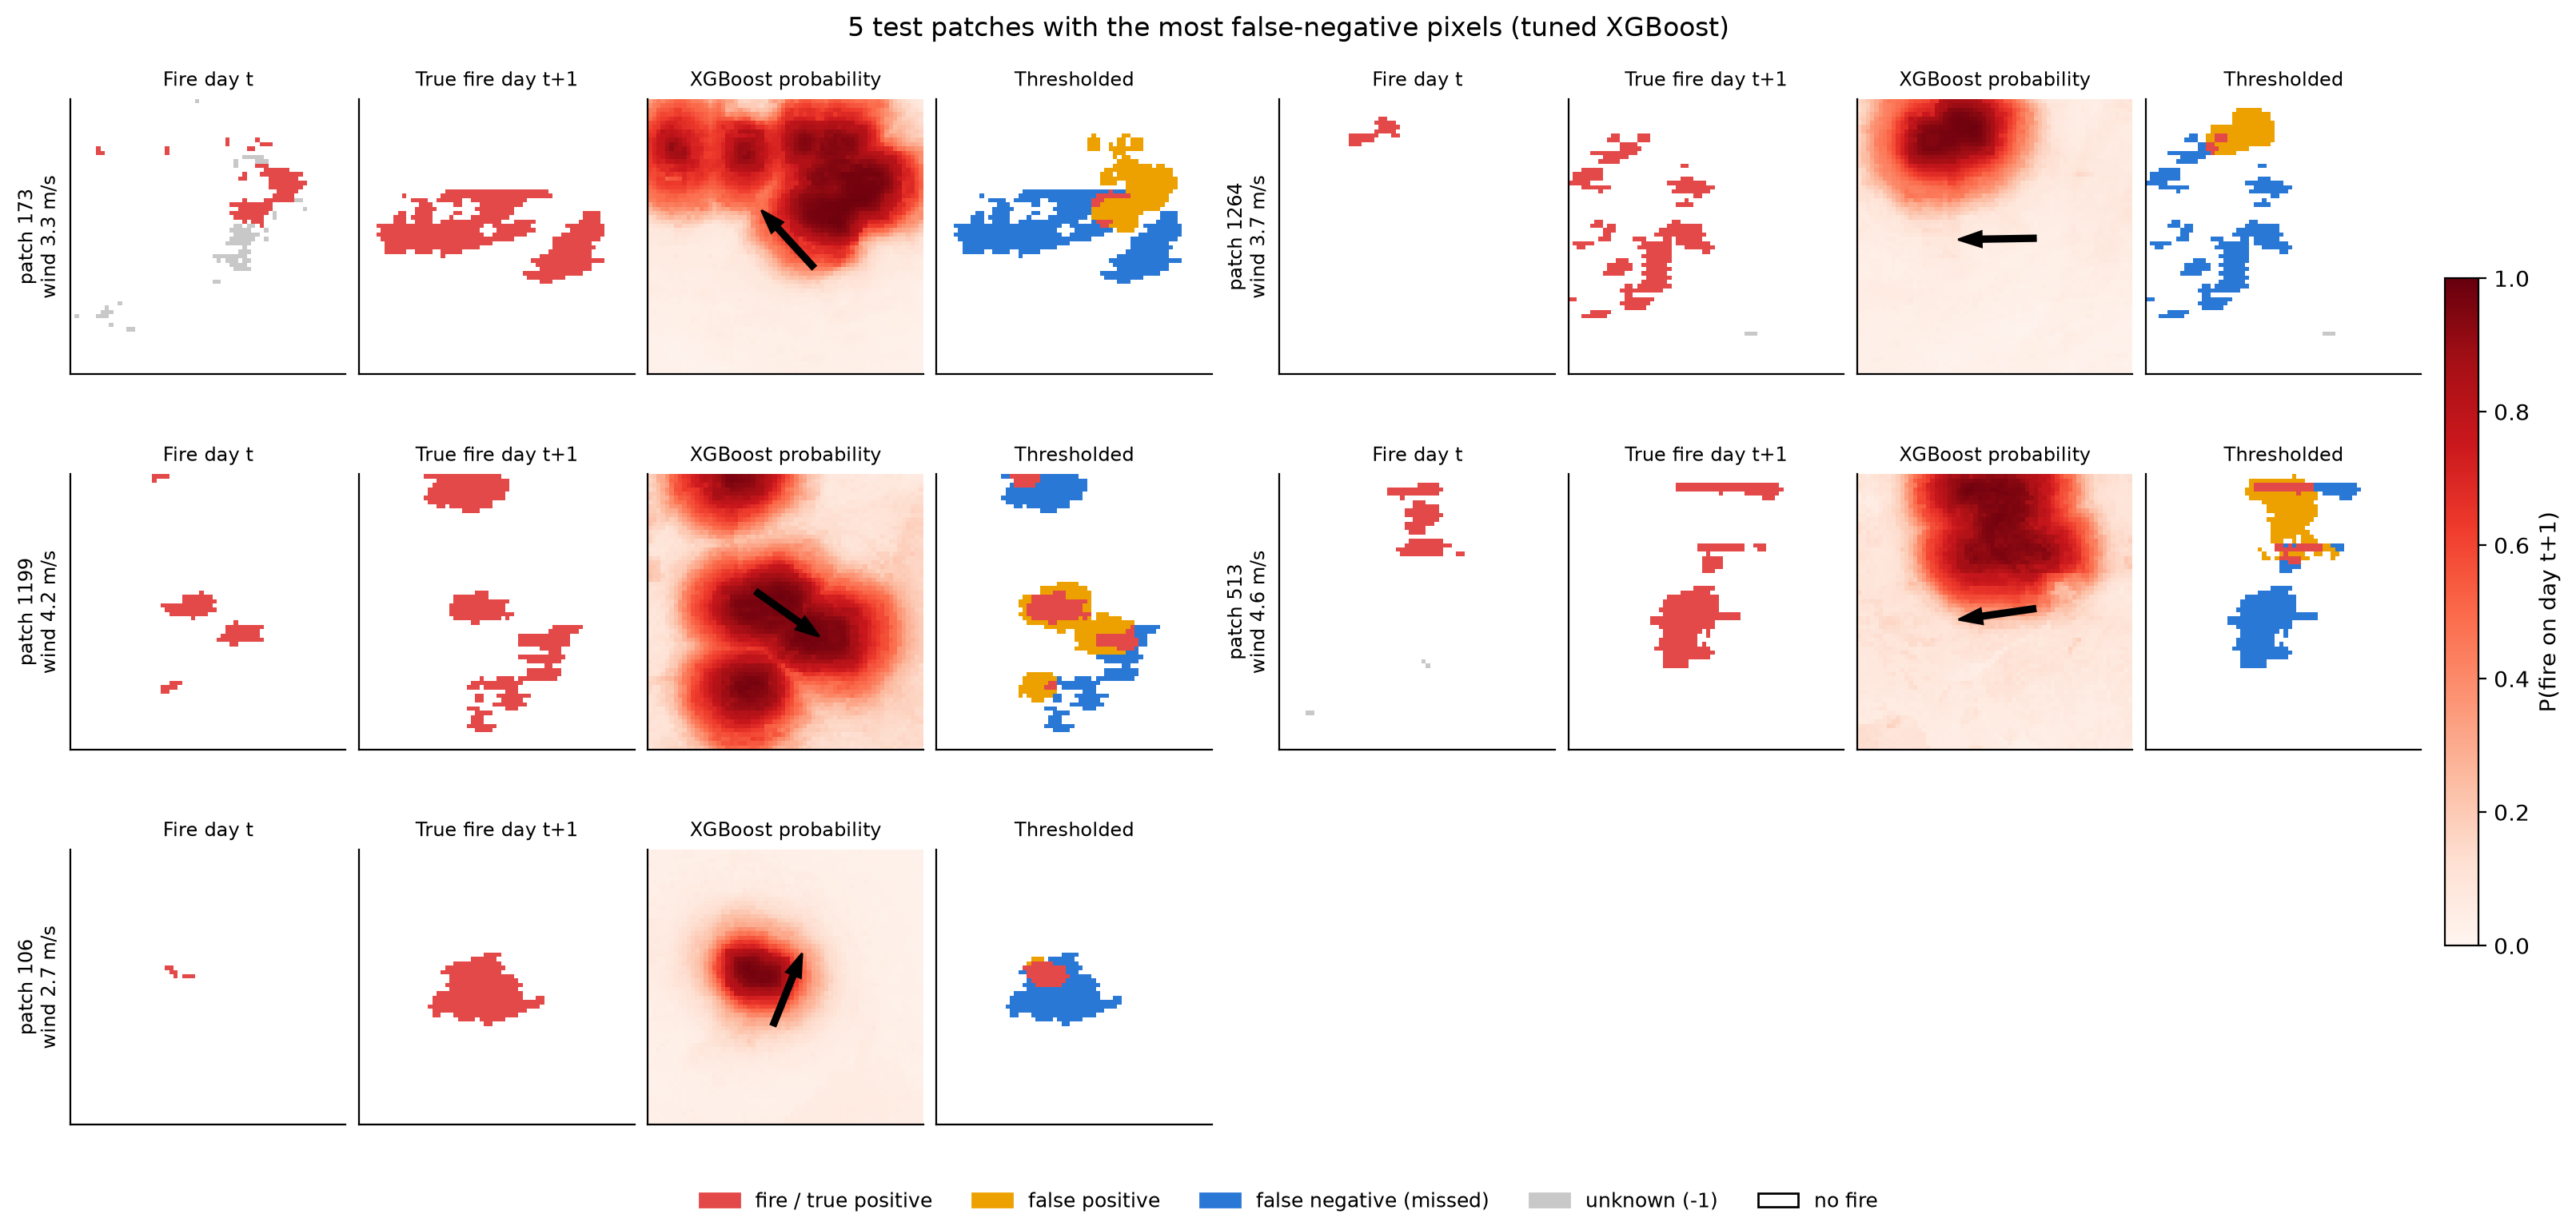
\includegraphics[width=0.49\textwidth]{figures/eval_worst_fn.png}
\caption{The five test patches (distinct locations) with the most false-positive (left) and false-negative (right)
pixels for the tuned XGBoost. Orange: false positive; blue: false negative; red: true positive.}
\label{fig:errors}
\end{figure*}

\begin{figure}[t]
\centering
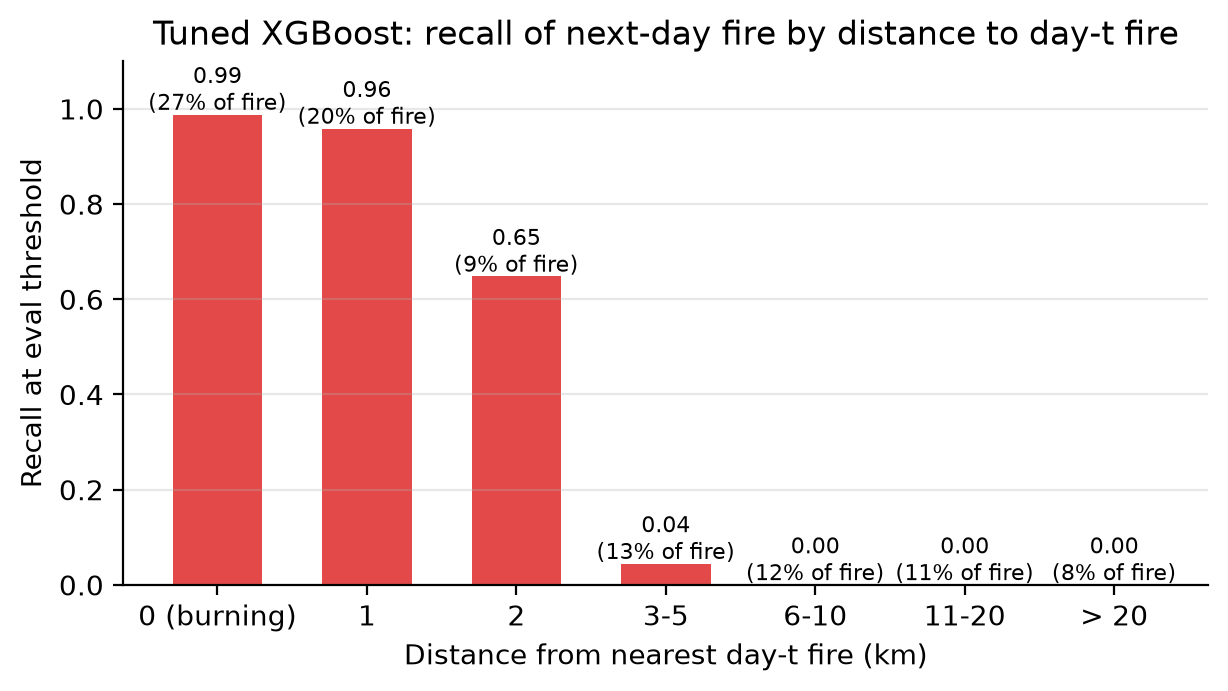
\includegraphics[width=\columnwidth]{figures/eval_recall_by_distance.png}
\caption{Recall of next-day fire pixels by distance to the nearest day-$t$ fire (tuned XGBoost, eval-chosen threshold).}
\label{fig:dist}
\end{figure}

\subsection{Limitations}
The test split contains 40 exact duplicate patches and overlapping crops of the same fires, so pixel-level metrics
weight large fires more than once; an event-level evaluation would be fairer. MODIS fire masks miss fire under cloud
and smoke, so part of the error is label noise. Finally, a per-pixel model with fixed-radius neighbourhood summaries
can only learn a fixed-radius halo; the remaining errors concern fire-front shape, long-range spread and whether a fire
grows or dies, which motivates the spatial models of Phase~2.
